\title{Perturbation Theory for Structural UQ}

% \author{
%         Anthony M. DeGennaro, Associate Computational Scientist, CSI
% }
\date{}

\documentclass[11pt]{article}
\usepackage[margin=1in]{geometry}
\usepackage{amsmath, amsfonts, bm, bbm, graphicx, caption, subcaption}
\usepackage{titling}
\usepackage{lipsum}
\setlength{\droptitle}{-0.75in}   % Adjust title margin
%% \pagenumbering{gobble}

\begin{document}
\newcommand*{\vertbar}{\rule[-1ex]{0.5pt}{2.5ex}}
\newcommand*{\horzbar}{\rule[.5ex]{2.5ex}{0.5pt}}
\maketitle

\vspace*{-0.75in}

\section{Review: Perturbation Theory}

The goal is to help mitigate the problem of structural UQ by using perturbation theory. 
We review the basics of perturbation theory here~\cite{khalil}.
Consider the equation:

\begin{equation}
        \label{eq:dynsys}
        \begin{aligned}
                \dot{u} &= f( u , t , \epsilon )  \\
                u &\in U \subset \mathbb{R}^n \;\;\; , \;\;\; t \in [t_0,t_f] \;\;\; , \;\;\; \epsilon \in [-\epsilon_0 , \epsilon_0].
        \end{aligned}
\end{equation}

\noindent We also allow for our initial conditions to depend smoothly on $\epsilon$:

\begin{equation}
        \label{eq:ics}
        u(t_0) = \eta(\epsilon) \;\;\; .
\end{equation}

\noindent Our goal is to quantify Eq.~\ref{eq:dynsys} over the distribution $\epsilon \sim \rho(\epsilon)$. 
The naive route is Monte Carlo sampling. 
However, one use of perturbation theory is to avoid this through separation of variables: we posit this expansion for the solution:

\begin{equation}
        \label{eq:expansion}
        \begin{aligned}
                u( t , \epsilon ) &\approx \sum_{k=0}^{N-1} u_k(t) \epsilon^k \\
                \eta( \epsilon ) &\approx \sum_{k=0}^{N-1} \eta_k \epsilon^k \;\;\; .
        \end{aligned}
\end{equation}

\noindent The fields $u_j(t)$ must be solved for through a system of ODEs obtained by substituting Eq.~\ref{eq:expansion} into Eq.~\ref{eq:dynsys} and matching terms in $\epsilon$:

\begin{equation}
        \label{eq:perteq}
        \begin{aligned}
                \dot{u}_0 &= f( t , u , 0 ) \;\;\; , \;\;\; u_0(t_0) = \eta_0 \\
                \dot{u}_k &= A(t) u_k + g_k( t , u_0(t) , \dots , u_{k-1}(t) ) \;\;\; , \;\;\; u_k(t_0) = \eta_k  \;\;\; ,
        \end{aligned}
\end{equation}

\noindent where $A(t) = [ \partial f / \partial u ]$ evaluated at $u_0(t)$.

\noindent The advantage for UQ is, we need only solve Eq.~\ref{eq:perteq} {\it once}. 
Then, we simply evaluate Eq.~\ref{eq:expansion} for any value of $\epsilon$ we like.

\section{Example: Van der Pol}

Consider this example:

\begin{equation}
        \label{eq:vdp}
        \begin{aligned}
                \dot{u}_1 &= u_2 \\
                \dot{u}_2 &= -u_1 + \epsilon ( 1 - u_1^2 ) u_2 \\
                \epsilon &\sim \mathcal{U}(-1,1) \\
                (u_1,u_2) &\sim \mathcal{U}(-2,2) \\
                t &\in [0,0.25] \;\;\; .
        \end{aligned}
\end{equation}

\noindent Fig.~\ref{fig:vdp_variations} plots the variations possible in this system with $\epsilon$.
In particular, we see the development of a nonlinear global attractor with increasing $\epsilon$.

\begin{figure}[h]
        \centering
        \begin{subfigure}{0.24\textwidth}
        \centering
                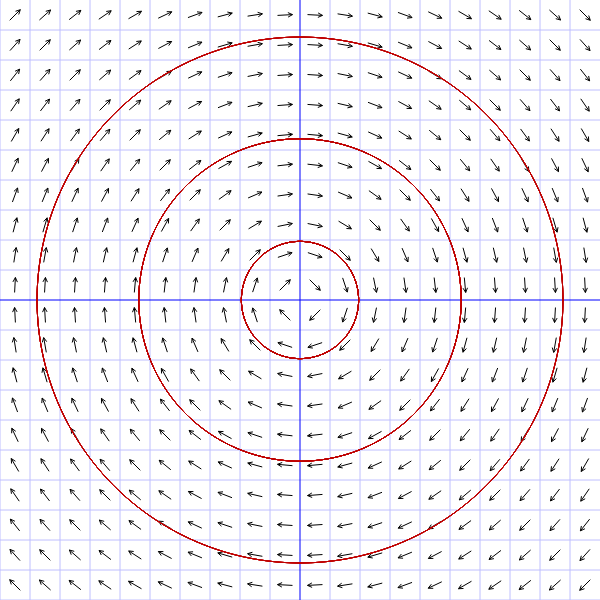
\includegraphics[width=0.95\linewidth]{vdp_0.png}
                \caption{$\epsilon = 0$.}
        \end{subfigure}
        \begin{subfigure}{0.24\textwidth}
        \centering
                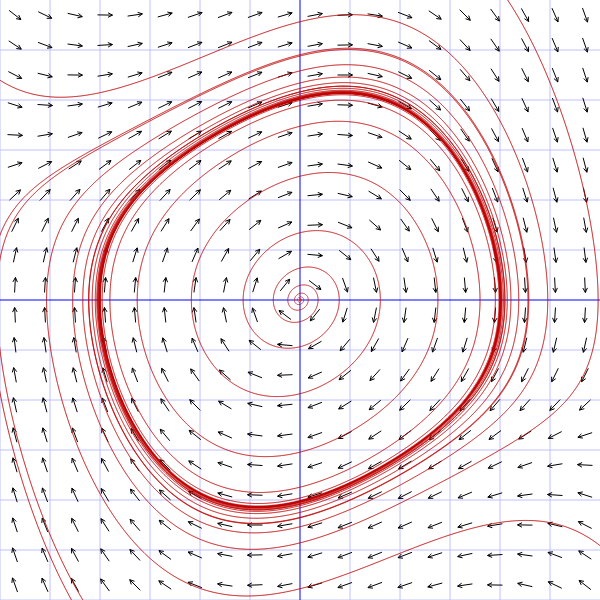
\includegraphics[width=0.95\linewidth]{vdp_0p25.png}
                \caption{$\epsilon = 0.25$.}
        \end{subfigure}
        \begin{subfigure}{0.24\textwidth}
        \centering
                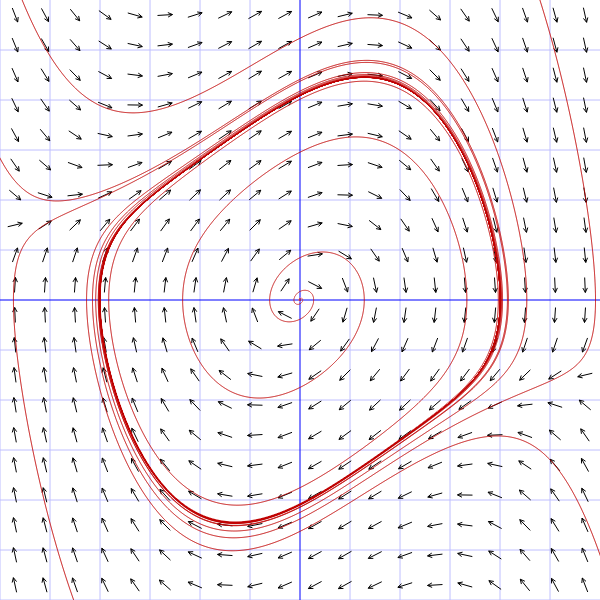
\includegraphics[width=0.95\linewidth]{vdp_0p5.png}
                \caption{$\epsilon = 0.5$.}
        \end{subfigure}
        \begin{subfigure}{0.24\textwidth}
        \centering
                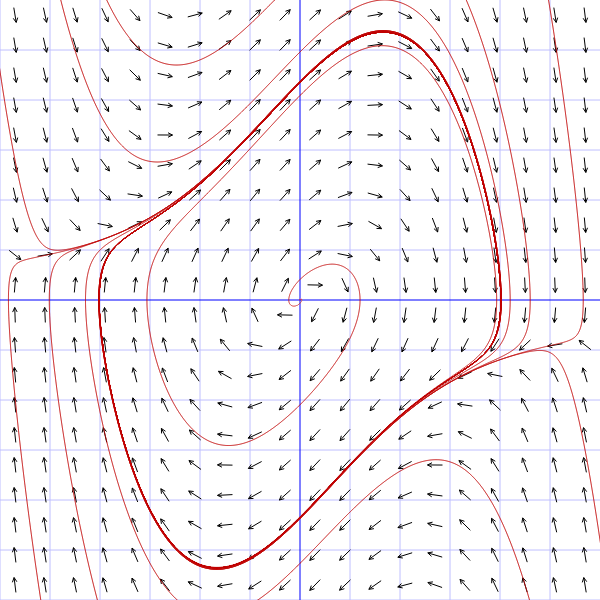
\includegraphics[width=0.95\linewidth]{vdp_1.png}
                \caption{$\epsilon = 1$.}
        \end{subfigure}                        
        \caption{Van der Pol equations for different values of $\epsilon$.}
        \label{fig:vdp_variations}
\end{figure}


\noindent We seek a perturbation expansion to approximate solution variation in $\epsilon$:

\begin{equation}
        \label{eq:vdp_exp}
        \begin{aligned}
                u_j &= u_{j0} + \epsilon u_{j1} + \epsilon^2 u_{j2}^2 \\
                \eta_j &= \eta_{j0} + \epsilon \eta_{j1} + \epsilon^2 \eta_{j2}^2 \;\;\; .
        \end{aligned}
\end{equation}

\noindent Substituting Eq.~\ref{eq:vdp_exp} into Eq.~\ref{eq:vdp} and matching $\mathcal{O}(1)$ terms gives the zeroth-order approximate system:

\begin{equation}
        \label{eq:zeroorder_vdp}
        \begin{aligned}
                \dot{u}_{10} &= u_{20} \;\;\; , \;\;\; u_{10} = u_1(t_0) \\
                \dot{u}_{20} &= -u_{10} \;\;\; , \;\;\; u_{20} = u_2(t_0) \;\;\; ,
        \end{aligned}
\end{equation}

\noindent which is the unperturbed ($\epsilon=0$) system.
Matching terms of $\mathcal{O}(\epsilon)$ gives the first-order approximate system:

\begin{equation}
        \label{eq:firstorder_vdp}
        \begin{aligned}
                \dot{u}_{11} &= u_{21} \;\;\; , \;\;\; u_{11} = 0 \\
                \dot{u}_{21} &= -u_{11} + ( 1 - u_{10}^2 ) u_{20} \;\;\; , \;\;\; u_{21} = 0 \;\;\; .
        \end{aligned}
\end{equation}

\noindent Likewise, $\mathcal{O}(\epsilon^2)$ gives:

\begin{equation}
        \label{eq:secondorder_vdp}
        \begin{aligned}
                \dot{u}_{12} &= u_{22} \;\;\; , \;\;\; u_{12} = 0 \\
                \dot{u}_{22} &= -u_{12} + ( 1 - u_{10}^2 ) u_{21} - 2 u_{10} u_{11} u_{20} \;\;\; , \;\;\; u_{22} = 0 \;\;\; .
        \end{aligned}
\end{equation}

\noindent Fig.~\ref{fig:vdp_vs_approx} shows the performance of the 2$^{\text{nd}}$-order approximate system against the full Van der Pol equations for $\epsilon=1$.
We again emphasize the independence of our approximate constructions from $\epsilon$: the fields $u_{jk}$ are obtained by solving one set of ODEs once, and then sampling over $\epsilon$ reduces to simple evaluation of Eq.~\ref{eq:vdp_exp}.
By contrast, naive sampling would involve solving a new system of ODEs for each and every value of $\epsilon$.

\begin{figure}[h]
        \centering
        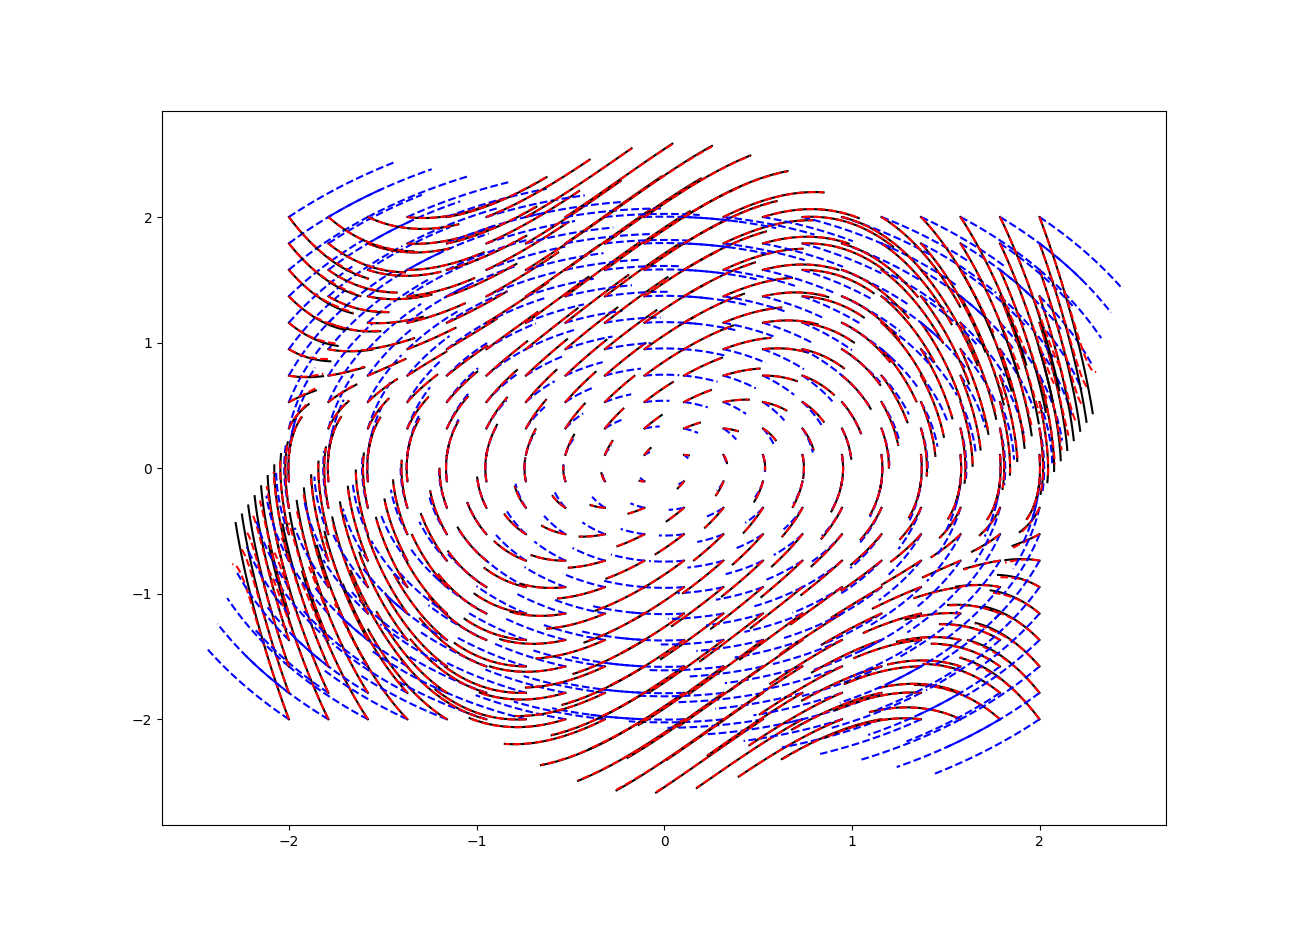
\includegraphics[width=0.6\textwidth]{vdp_vs_approx_eps1.png}
        \caption{Comparison of Van der Pol (black), 0$^{\text{th}}$-order (blue), and 2$^{\text{nd}}$-order (red) approximate systems for $\epsilon=1$.}
        \label{fig:vdp_vs_approx}
\end{figure}



\section*{}
%\vspace*{-0.75in}
\newpage
\bibliographystyle{plain}
\bibliography{notes.bib}


\end{document}
